% schematic for PEC and interface reactions for MRS2019 meet-faculty candidate
% adapted from:http://www.texample.net/tikz/examples/clusters-of-atoms/

% Clusters of atoms
% Adapted and modified: wwwennie
% Author: Agustin E. Bolzan
\documentclass{article}
\usepackage[rgb]{xcolor}
\usepackage{tikz,pgffor}
\usetikzlibrary{shadows,fadings}
\begin{document}


%\begin{figure}
\centering
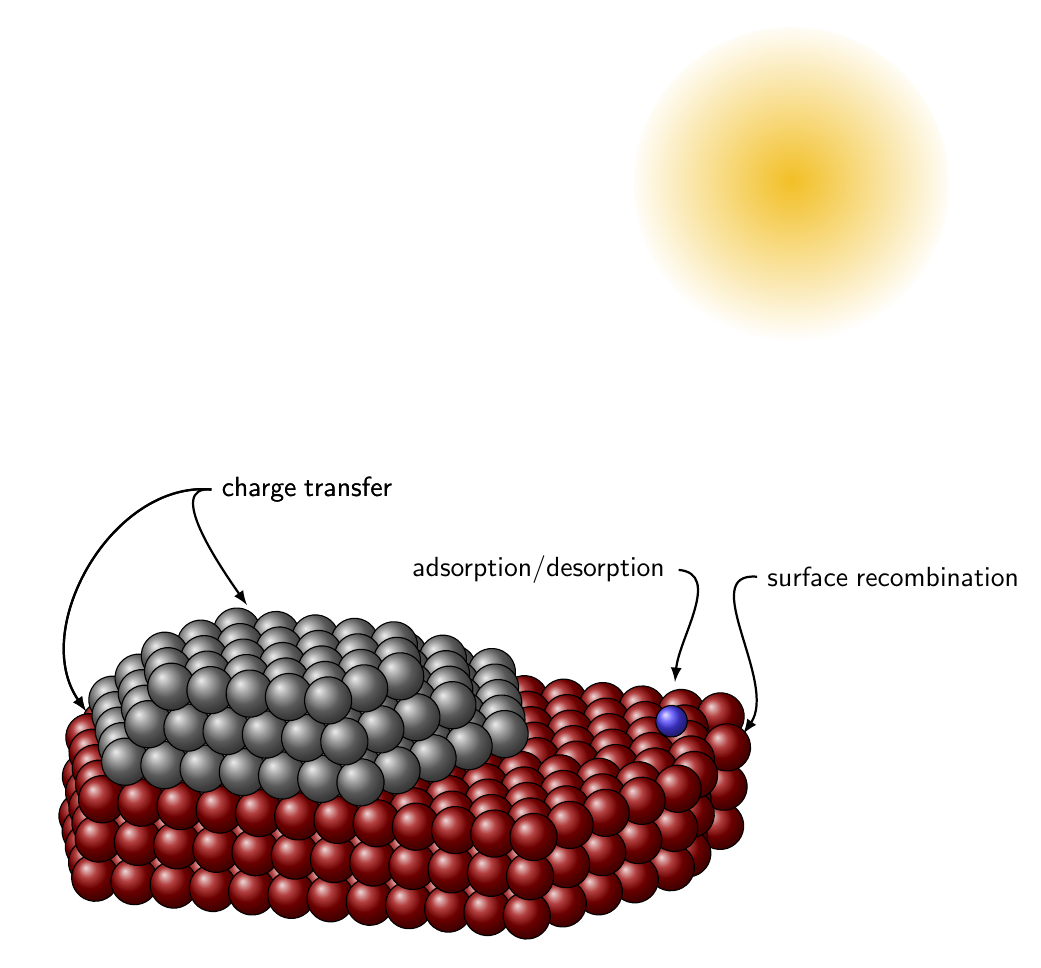
\begin{tikzpicture}
%\draw[help lines] (0,0) grid (10,10); %used just for visualising the positions of objects during construction
%
% \begin{scope}[yshift=-180,yslant=0.5,xslant=-1]
%     %the rectangular surface onto which the clusters are located
%     \filldraw[black!10,very thick] (0.5,1) rectangle (10,7);
%     %circle circumventing the smallest cluster
%     \node[circle,circular glow,fill=maroon!20,draw=maroon,thick]
%     at (4.1,4.9) {\phantom{perimetro}};
% \end{scope}

%atom clusters are rotated for a better visualisation
\begin{scope}[rotate around = {-5:(0,0,0)}]
    %%% text describing the objects in the picture
    % \draw[-latex,thick] (6,3) node[right,text width=3cm]
    %     {$\mathsf{potent\; perimeter\; sites}$} to [out=180,in=0] (5.5,1);
    % \draw[-latex,thick](3,-1)node[right]
    %     {$\mathsf{Non-metallic\; molecule}$} to[out=180,in=0] (2.6,-3);
    % \draw[-latex,thick](-3,-1)node[above]
    %     {$\mathsf{extra \; electron}$} to[out=-90,in=180] (-1.4,-2);

    %now we start with the clusters (maybe this code could be improved by a tikz expert)
    %the layers are built starting from the very lowest one

    % user-defined parameters
    \pgfmathsetmacro{\ballsize}{0.3}
    \definecolor{maroon}{rgb}{0.6,0.0,0.0}
    \definecolor{violet}{rgb}{0.3,0.25,1.0}
    \definecolor{darkyellow}{rgb}{0.95,0.75,0.15}

    %largest cluster
    %extra bottom rows for material 1
    \foreach \x  in {1.5,2,2.5,3,3.5,4,4.5,5.0,5.5,6.0,6.5,7.0,7.5}%
        \shadedraw [ball color= maroon] (\x,0.0,-0.5) circle (\ballsize cm);
    \foreach \x  in {1.25,1.75,2.25,2.75,3.25,3.75,4.25,4.75,5.25,5.75,6.25,6.75,7.25}%
        \shadedraw [ball color= maroon] (\x,0.0,0.0) circle (\ballsize cm);
    \foreach \x  in {1,1.5,2,2.5,3,3.5,4,4.5,5.0,5.5,6.0,6.5,7.0,7.5,8.0}%
        \shadedraw [ball color= maroon] (\x,0.0,0.5) circle (\ballsize cm);
    \foreach \x  in {0.75,1.25,1.75,2.25,2.75,3.25,3.75,4.25,4.75,5.25,5.75,6.25,6.75,7.25,7.75}%
        \shadedraw [ball color= maroon] (\x,0.0,1) circle (\ballsize cm);
    \foreach \x  in {0.5,1,1.5,2,2.5,3,3.5,4,4.5,5,5.5,6.0,6.5,7.0,7.5,8.0}%
        \shadedraw [ball color= maroon] (\x,0.0,1.5) circle (\ballsize cm);
    \foreach \x  in {0.5,1,1.5,2,2.5,3,3.5,4,4.5,5,5.5,6.0,6.5,7.0,7.5,8.0}
        \shadedraw [ball color=maroon] (\x,0.0,2) circle (\ballsize cm);
    \foreach \x  in {0.75,1.25,1.75,2.25,2.75,3.25,3.75,4.25,4.75,5.25,5.75,6.25,6.75,7.25,7.75}%
        \shadedraw [ball color= maroon] (\x,0.0,2.5) circle (\ballsize cm);
    \foreach \x  in {1,1.5,2,2.5,3,3.5,4,4.5,5,5.5,6.0,6.5,7.0,7.5}%
        \shadedraw [ball color= maroon] (\x,0.0,3) circle (\ballsize cm);
    \foreach \x  in {1.25,1.75,2.25,2.75,3.25,3.75,4.25,4.75,5.25,5.75,6.25,6.75,7.25}%
        \shadedraw [ball color= maroon] (\x,0.0,3.5) circle (\ballsize cm);
    \foreach \x  in {1.5,2,2.5,3,3.5,4,4.5,5.0,5.5,6.0,6.5,7.0}%
        \shadedraw [ball color= maroon] (\x,0.0,4.0) circle (\ballsize cm);
    %
    %extra bottom rows for material 1
    \foreach \x  in {1.5,2,2.5,3,3.5,4,4.5,5.0,5.5,6.0,6.5,7.0,7.5}%
        \shadedraw [ball color= maroon] (\x,0.5,-0.5) circle (\ballsize cm);
    \foreach \x  in {1.25,1.75,2.25,2.75,3.25,3.75,4.25,4.75,5.25,5.75,6.25,6.75,7.25}%
        \shadedraw [ball color= maroon] (\x,0.5,0.0) circle (\ballsize cm);
    \foreach \x  in {1,1.5,2,2.5,3,3.5,4,4.5,5.0,5.5,6.0,6.5,7.0,7.5,8.0}%
        \shadedraw [ball color= maroon] (\x,0.5,0.5) circle (\ballsize cm);
    \foreach \x  in {0.75,1.25,1.75,2.25,2.75,3.25,3.75,4.25,4.75,5.25,5.75,6.25,6.75,7.25,7.75}%
        \shadedraw [ball color= maroon] (\x,0.5,1) circle (\ballsize cm);
    \foreach \x  in {0.5,1,1.5,2,2.5,3,3.5,4,4.5,5,5.5,6.0,6.5,7.0,7.5,8.0}%
        \shadedraw [ball color= maroon] (\x,0.5,1.5) circle (\ballsize cm);
    \foreach \x  in {0.5,1,1.5,2,2.5,3,3.5,4,4.5,5,5.5,6.0,6.5,7.0,7.5,8.0}
        \shadedraw [ball color=maroon] (\x,0.5,2) circle (\ballsize cm);
    \foreach \x  in {0.75,1.25,1.75,2.25,2.75,3.25,3.75,4.25,4.75,5.25,5.75,6.25,6.75,7.25,7.75}%
        \shadedraw [ball color= maroon] (\x,0.5,2.5) circle (\ballsize cm);
    \foreach \x  in {1,1.5,2,2.5,3,3.5,4,4.5,5,5.5,6.0,6.5,7.0,7.5}%
        \shadedraw [ball color= maroon] (\x,0.5,3) circle (\ballsize cm);
    \foreach \x  in {1.25,1.75,2.25,2.75,3.25,3.75,4.25,4.75,5.25,5.75,6.25,6.75,7.25}%
        \shadedraw [ball color= maroon] (\x,0.5,3.5) circle (\ballsize cm);
    \foreach \x  in {1.5,2,2.5,3,3.5,4,4.5,5.0,5.5,6.0,6.5,7.0}%
        \shadedraw [ball color= maroon] (\x,0.5,4.0) circle (\ballsize cm);
    %

    %first row
    \foreach \x  in {1.5,2,2.5,3,3.5,4,4.5,5.0,5.5,6.0,6.5,7.0,7.5}%
        \shadedraw [ball color= maroon] (\x,1,-0.5) circle (\ballsize cm);
    \foreach \x  in {1.25,1.75,2.25,2.75,3.25,3.75,4.25,4.75,5.25,5.75,6.25,6.75,7.25}%
        \shadedraw [ball color= maroon] (\x,1,0.0) circle (\ballsize cm);
    \foreach \x  in {1,1.5,2,2.5,3,3.5,4,4.5,5.0,5.5,6.0,6.5,7.0,7.5,8.0}%
        \shadedraw [ball color= maroon] (\x,1,0.5) circle (\ballsize cm);
    \foreach \x  in {0.75,1.25,1.75,2.25,2.75,3.25,3.75,4.25,4.75,5.25,5.75,6.25,6.75,7.25,7.75}%
        \shadedraw [ball color= maroon] (\x,1,1) circle (\ballsize cm);
    \foreach \x  in {0.5,1,1.5,2,2.5,3,3.5,4,4.5,5,5.5,6.0,6.5,7.0,7.5,8.0}%
        \shadedraw [ball color= maroon] (\x,1,1.5) circle (\ballsize cm);
    \foreach \x  in {0.5,1,1.5,2,2.5,3,3.5,4,4.5,5,5.5,6.0,6.5,7.0,7.5,8.0}
        \shadedraw [ball color=maroon] (\x,1,2) circle (\ballsize cm);
    \foreach \x  in {0.75,1.25,1.75,2.25,2.75,3.25,3.75,4.25,4.75,5.25,5.75,6.25,6.75,7.25,7.75}%
        \shadedraw [ball color= maroon] (\x,1,2.5) circle (\ballsize cm);
    \foreach \x  in {1,1.5,2,2.5,3,3.5,4,4.5,5,5.5,6.0,6.5,7.0,7.5}%
        \shadedraw [ball color= maroon] (\x,1,3) circle (\ballsize cm);
    \foreach \x  in {1.25,1.75,2.25,2.75,3.25,3.75,4.25,4.75,5.25,5.75,6.25,6.75,7.25}%
        \shadedraw [ball color= maroon] (\x,1,3.5) circle (\ballsize cm);
    \foreach \x  in {1.5,2,2.5,3,3.5,4,4.5,5.0,5.5,6.0,6.5,7.0}%
        \shadedraw [ball color= maroon] (\x,1,4.0) circle (\ballsize cm);

    %second row
    \foreach \x  in {1.75,2.25,2.75,3.25,3.75,4.25,4.75}
        \shadedraw [ball color=gray] (\x,1.5,0) circle (\ballsize cm);
    \foreach \x  in {1.5,2,2.5,3,3.5,4,4.5,5}
        \shadedraw [ball color=gray] (\x,1.5,0.5) circle (\ballsize cm);
    \foreach \x  in {1.25,1.75,2.25,2.75,3.25,3.75,4.25,4.75,5.25}
        \shadedraw [ball color=gray] (\x,1.5,1) circle (\ballsize cm);
    \foreach \x  in {1,1.5,2,2.5,3,3.5,4,4.5,5,5.5}
        \shadedraw [ball color=gray] (\x,1.5,1.5) circle (\ballsize cm);
    \foreach \x  in {0.75,1.25,1.75,2.25,2.75,3.25,3.75,4.25,4.75,5.25,5.75}
        \shadedraw [ball color=gray] (\x,1.5,2) circle (\ballsize cm);
    \foreach \x  in {1,1.5,2,2.5,3,3.5,4,4.5,5,5.5}
        \shadedraw [ball color=gray] (\x,1.5,2.5) circle (\ballsize cm);
    \foreach \x  in {1.25,1.75,2.25,2.75,3.25,3.75,4.25,4.75,5.25}
        \shadedraw [ball color=gray] (\x,1.5,3) circle (\ballsize cm);
    \foreach \x  in {1.5,2,2.5,3,3.5,4,4.5,5}
        \shadedraw [ball color=gray] (\x,1.5,3.5) circle (\ballsize cm);
    \foreach \x  in {1.75,2.25,2.75,3.25,3.75,4.25,4.75}
        \shadedraw [ball color=gray] (\x,1.5,4) circle (\ballsize cm);
    %third row
    \foreach \x  in {2,2.5,3,3.5,4,4.5}
        \shadedraw [ball color=gray] (\x,2,1) circle (\ballsize cm);
    \foreach \x  in {1.75,2.25,2.75,3.25,3.75,4.25,4.75}
        \shadedraw [ball color=gray] (\x,2,1.5) circle (\ballsize cm);
    \foreach \x  in {1.5,2,2.5,3,3.5,4,4.5,5}
        \shadedraw [ball color=gray] (\x,2,2) circle (\ballsize cm);
    \foreach \x  in {1.25,1.75,2.25,2.75,3.5,3.75,4.25,4.75,5.25}
        \shadedraw [ball color=gray] (\x,2,2.5) circle (\ballsize cm);
    \foreach \x  in {1.5,2,2.5,3,3.5,4,4.5,5}
        \shadedraw [ball color=gray] (\x,2,3) circle (\ballsize cm);
    \foreach \x  in {1.75,2.25,2.75,3.25,3.75,4.25,4.75}
        \shadedraw [ball color=gray] (\x,2,3.5) circle (\ballsize cm);
    \foreach \x  in {2,2.5,3,3.5,4,4.5}
        \shadedraw [ball color=gray] (\x,2,4) circle (\ballsize cm);
    %fourth row
    \foreach \x  in {2.25,2.75,3.25,3.75,4.25}
        \shadedraw [ball color=gray] (\x,2.5,2) circle (\ballsize cm);
    \foreach \x  in {2,2.5,3,3.5,4,4.5}
        \shadedraw [ball color=gray] (\x,2.5,2.5) circle (\ballsize cm);
    \foreach \x  in {1.75,2.25,2.75,3.25,3.75,4.25,4.75}
        \shadedraw [ball color=gray] (\x,2.5,3) circle (\ballsize cm);
    \foreach \x  in {2,2.5,3,3.5,4,4.5}
        \shadedraw [ball color=gray] (\x,2.5,3.5) circle (\ballsize cm);
    \foreach \x  in {2.25,2.75,3.25,3.75,4.25}
        \shadedraw [ball color=gray] (\x,2.5,4) circle (\ballsize cm);

    %adsorbed molecule
    \shadedraw [ball color= violet] (6.5,0.5,-1.5) circle (0.2 cm);
    % self-added text and arrow describing different interfacial and surface phenomena
    \draw[-latex,thick] (8,3) node[right,text width=3cm]
        {$\mathsf{surface\; recombination}$} to [out=180,in=60] (8.0,1);
    \draw[-latex,thick] (7,3) node[left,text width=3.25cm]
            {$\mathsf{adsorption/desorption}$} to [out=0,in=90] (6.5,1,-1.5);
    \draw[-latex,thick] (1,3.5) node[right,text width=3cm]
            {$\mathsf{charge\; transfer}$} to [out=180,in=130] (-0.15,0.75,0.5);
    \draw[-latex,thick] (1,3.5) node[right,text width=3cm]
            {$\mathsf{charge\; transfer}$} to [out=180,in=130] (-0.15,0.75,0.5);
    \draw[-latex,thick] (1,3.5) to [out=180,in=130] (1,1.5,-1.5);
    %the sun
    \shade [inner color=darkyellow,outer color=white] (8,8) circle (2 cm);

    %%% call out atoms and arrows
    % %medium cluster
    % %first row
    % \foreach \x  in {6.75,7.25}
    %     \shadedraw [ball color=gray] (\x,2.5,13) circle (0.25cm);
    % \foreach \x  in {6.5,7,7.5}
    %     \shadedraw [ball color=gray] (\x,2.5,13.5) circle (0.25cm);
    % \foreach \x  in {6.25,6.75,7.25,7.75}
    %     \shadedraw [ball color=gray] (\x,2.5,14) circle (0.25cm);
    % \foreach \x  in {6.5,7,7.5}
    %     \shadedraw [ball color=gray] (\x,2.5,14.5) circle (0.25cm);
    % \foreach \x  in {6.75,7.25}
    %     \shadedraw [ball color=gray] (\x,2.5,15) circle (0.25);
    %
    % %second row
    % \foreach \x  in {7} %this foreach is used to be general, but it makes no sense if we put just one sphere!
    %     \shadedraw [ball color=gray] (\x,3,13.25) circle (0.25cm);
    % \foreach \x  in {6.75,7.25}
    %     \shadedraw [ball color=gray] (\x,3,13.75) circle (0.25cm);
    % \foreach \x  in {6.5,7,7.5}
    %     \shadedraw [ball color=gray] (\x,3,14.25) circle (0.25cm);
    % \foreach \x  in {6.75,7.25}
    %     \shadedraw [ball color=gray] (\x,3,14.75) circle (0.25cm);
    % \foreach \x  in {7}
    %     \shadedraw [ball color=gray] (\x,3,15.25) circle (0.25);
    %
    % %smallest cluster of atoms
    %
    % \foreach \x in {2.75,3.25,3.75}
    %     \shadedraw [ball color = gray] (\x,2,10) circle (0.25);
    % \foreach \x in {3,3.5}
    %     \shadedraw [ball color=gray] (\x,2,10.5) circle (0.25);
    % \shadedraw [ball color = gray] (3.25,2,11) circle (0.25);
    % \foreach \x in {3,3.5}
    %     \shadedraw [ball color = gray] (3,2.5,10.25) circle (0.25);
    % \shadedraw [ball color = gray] (3.5,2.5,11) circle (0.25);

    % \shadedraw [ball color=maroon] (2,1,12.5) circle(0.25);
    % \draw[-latex,thick](-4,-3)node[above]
    %     {$\mathsf{single \; metal\; atom}$} to[out=-90,in=180] (-3,-4);
\end{scope}

% % pseudo-water
% \begin{scope}[yslant=0.0,xslant=0]
%    \tikzfading[name=fade vertical,
%     bottom color=transparent!0, top color=transparent!100]
%     %the rectangular surface onto which the clusters are located
%     \fill[blue,path fading=fade vertical,opacity=0.1] (-1,-3) rectangle (12,6);
% \end{scope}

\end{tikzpicture}
%\end{figure}
\end{document}
